\label{sec:5.1}

%%%%%%%%%%%%%%%%%%%%%%%%%%%%%%%%%%%%%%%%%%%%%%%%%%%
% Autocal
%%%%%%%%%%%%%%%%%%%%%%%%%%%%%%%%%%%%%%%%%%%%%%%%%%%

The linearity of the ADC is primarily determined by the capacitor matching internal to the circuit, and to a lesser extent the performance of the internal amplifiers. To achieve the target specifications, the ADC requires calibration. The calibration in ColdADC can be carried out internally, in a fully automated way, or can be done externally. Unfortunately, while the chip can be fully calibrated externally, with calibration data loaded back onto the chip, the autocal function failed in the prototype. The ADC performance under autocal or external calibration does not differ in any way, so the main issue here is the loss of convenience that autocal promises.

When we developed the digital part of the ColdADC, we decided to partition the blocks such that the blocks that calibrate the ADC and compute the corrected digital output would be placed within the ADC cores, and the rest of the digital logic would be aggregated in a third core. This can be seen in Figure~\ref{fig:autocalBlock}. The CAL\_UNIT is the block that performs the calibration and also applies the calibration coefficients (or weights) to the data during normal operation. Each CAL\_UNIT stores the calculated configuration weights to the register file in the CAL\_CORE (which was synthesized separately).
\begin{figure}[h]
\centering
%\begin{minipage}[b]{1.0\textwidth}
\begin{center}
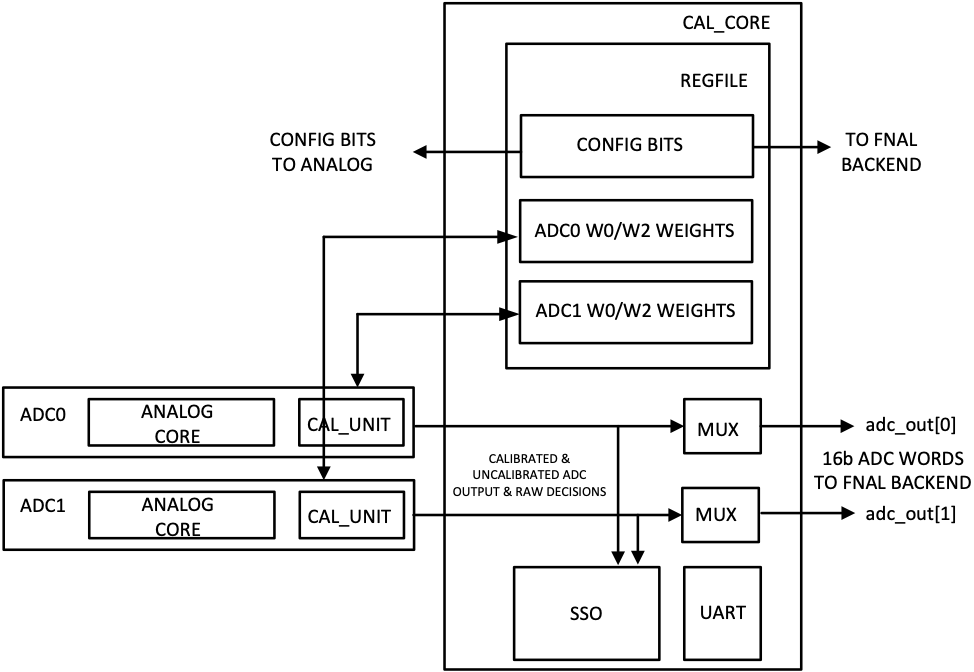
\includegraphics[width=0.8\textwidth]{figures/autocalBlock.png}
\end{center}
%\end{minipage}
\caption{Partitioning of Digital Logic in the ColdADC.}
\label{fig:autocalBlock}
\end{figure}

This would have been an acceptable strategy but due to miscommunication the interface between the cores was not simulated with back-annotated timing. This means that the timing when a computed calibration coefficient is written back into the registers was not simulated properly. When the blocks were placed, there was a timing error between the CAL\_UNIT and the CAL\_CORE in the case when the CAL\_UNIT was writing back computed calibration weights into storage in the CAL\_CORE.

An example of the intended operation is shown in Figure~\ref{fig:correctcalwrite}. In this simulation the CAL\_UNIT is back annotated with parasitics (but the interface with the CAL\_CORE is not properly back annotated). In this simulation, the intended data is in the second row (the word 0x03FD) and is written to the w2\_4 register that resides in the CAL\_CORE correctly. Correct operation is assured by disabling the memory after the edge of clk.
\begin{figure}[h]
\centering
%\begin{minipage}[b]{1.0\textwidth}
\begin{center}
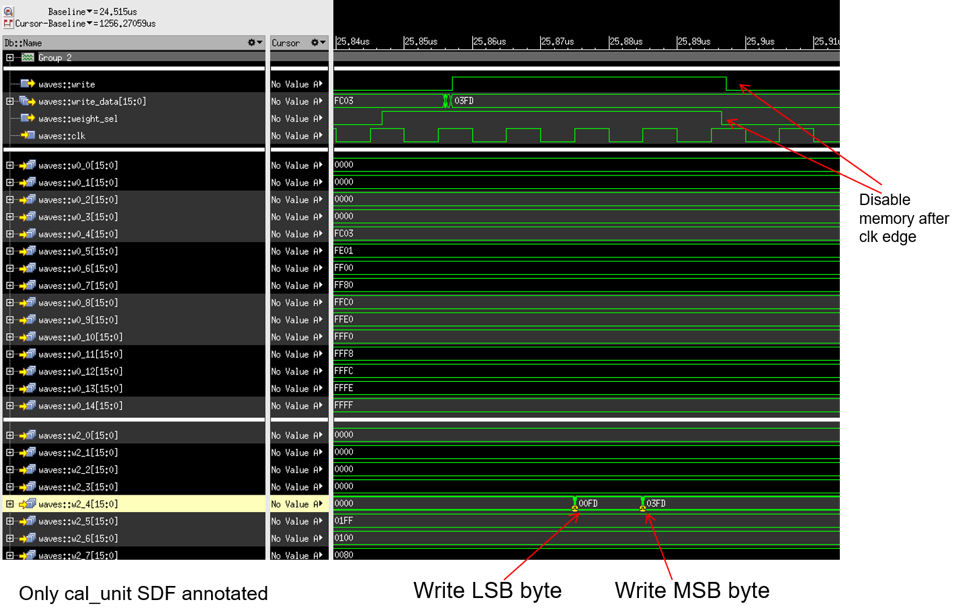
\includegraphics[width=1.0\textwidth]{figures/CorrectCalWrite.png}
\end{center}
%\end{minipage}
\caption{Correct writeback of calibration weights}
\label{fig:correctcalwrite}
\end{figure}

When the interface between CAL\_UNIT and CAL\_CORE was properly annotated and simulated, the result was in Figure~\ref{fig:errorcalwrite}.
\begin{figure}[htb]
\centering
%\begin{minipage}[b]{1.0\textwidth}
\begin{center}
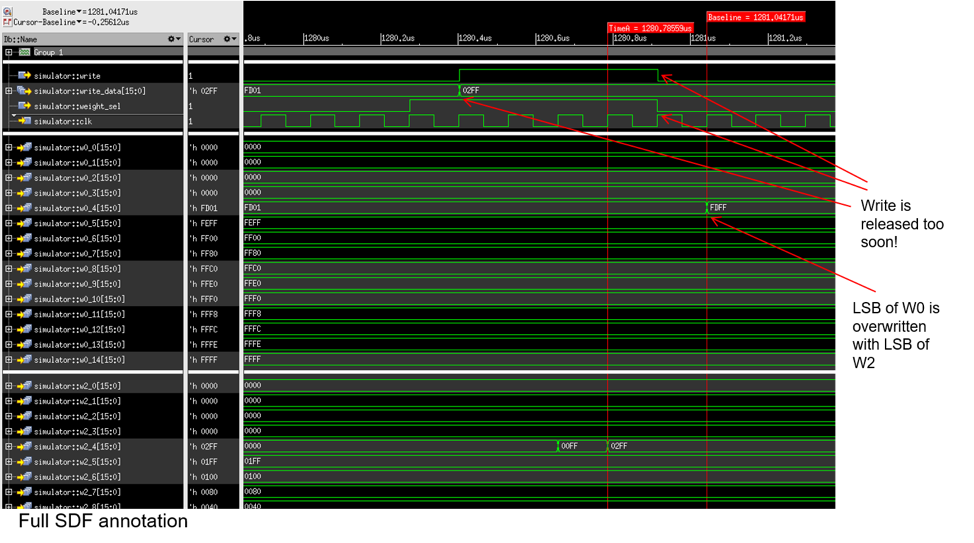
\includegraphics[width=1.0\textwidth]{figures/ErrorCalWrite.png}
\end{center}
%\end{minipage}
\caption{Error in writeback of calibration weights}
\label{fig:errorcalwrite}
\end{figure}

A gross error has been made, because the write signal is released too soon and therefore we have a race condition. What happens specifically here is that due to the race condition, the LSB byte of w0[4] is overwritten with the LSB byte of w2[4]. This is error and causes the entire calibration sequence to fail.

The fix here is to repartition the digital logic for the second version of the ColdADC ASIC. We will move the digital calibration and correction logic out of the ADCs and into a single, monolithic digital block as shown in Figure~\ref{fig:autocalBlock_new}. This will ensure that the interfaces between the calculation engines and the memory are simulated correctly and the absence of race conditions will be verified using static timing analysis. The RTL code itself will also be made more robust by adjusting the internal state machine.
\begin{figure}[h]
\centering
%\begin{minipage}[b]{1.0\textwidth}
\begin{center}
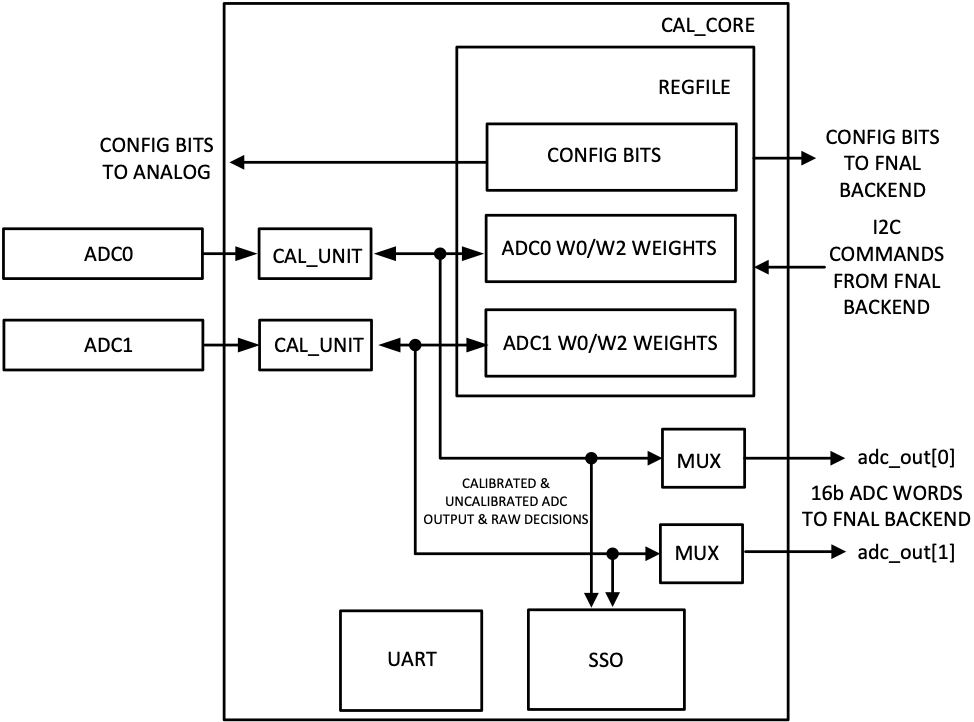
\includegraphics[width=0.8\textwidth]{figures/autocalBlock_new.png}
\end{center}
%\end{minipage}
\caption{Proposed Calibration Digital Logic partitioning in revised prototype.}
\label{fig:autocalBlock_new}
\end{figure}

